\section{Hamiltonian Monte Carlo}
\label{sec:HMC}
A very popular MCMC method is the Hamiltonian Monte Carlo (or Hybrid Monte Carlo, HMC) algorithm \parencite{Duane1987}, since it is highly efficient and widely applicable. The idea behind this algorithm is to propose new points by simulating the dynamics of a particle on a potential energy landscape induced by the desired target distribution. This simulation is done using the Hamiltonian Dynamics formulation, which results in several useful properties for the HMC algorithm. These can be further exploited by using HMC within the MCVI scheme. To understand these synergies, we will first review Hamiltonian Dynamics and the HMC algorithm. For a more exhaustive review and discussion refer to \textcite{Neal2011}.

\subsection{Hamiltonian Dynamics}

Hamiltonian Dynamics (HD) is a reformulation of classical dynamics, where the state of the physical system is described by a pair $(q, p)$ of $d$-dimensional vectors, where $q$ is the \textit{position} vector and $p$ is the \textit{momentum} vector. The evolution of the system with time is then given by \textit{Hamilton's equations}:
\begin{equation} \label{eq:HamiltonsEquations}
\begin{split}
\frac{dq_i}{dt} &= \frac{\partial H}{\partial p_i} \\
\frac{dp_i}{dt} &= - \frac{\partial H}{\partial q_i},
\end{split}
\end{equation}
where $H(q, p, t)$ is the \textit{Hamiltonian} of the system (often its total energy).

For our application, we are interested in the motion of a frictionless particle governed by the \textit{potential energy} $U(q)$ and \textit{kinetic energy} $K(p)$. In this setting the Hamiltonian is just the total energy of the system, i.e.\ $H(q, p) = U(q) + K(p)$, which is independent of time due to conservation of energy. In two dimensions this can be visualized well as a frictionless particle sliding over a landscape of varying height (see figure~\ref{fig:HMC_MOTION_1hmc_12lf} for a numerically solved example).

\begin{figure*}
\centering
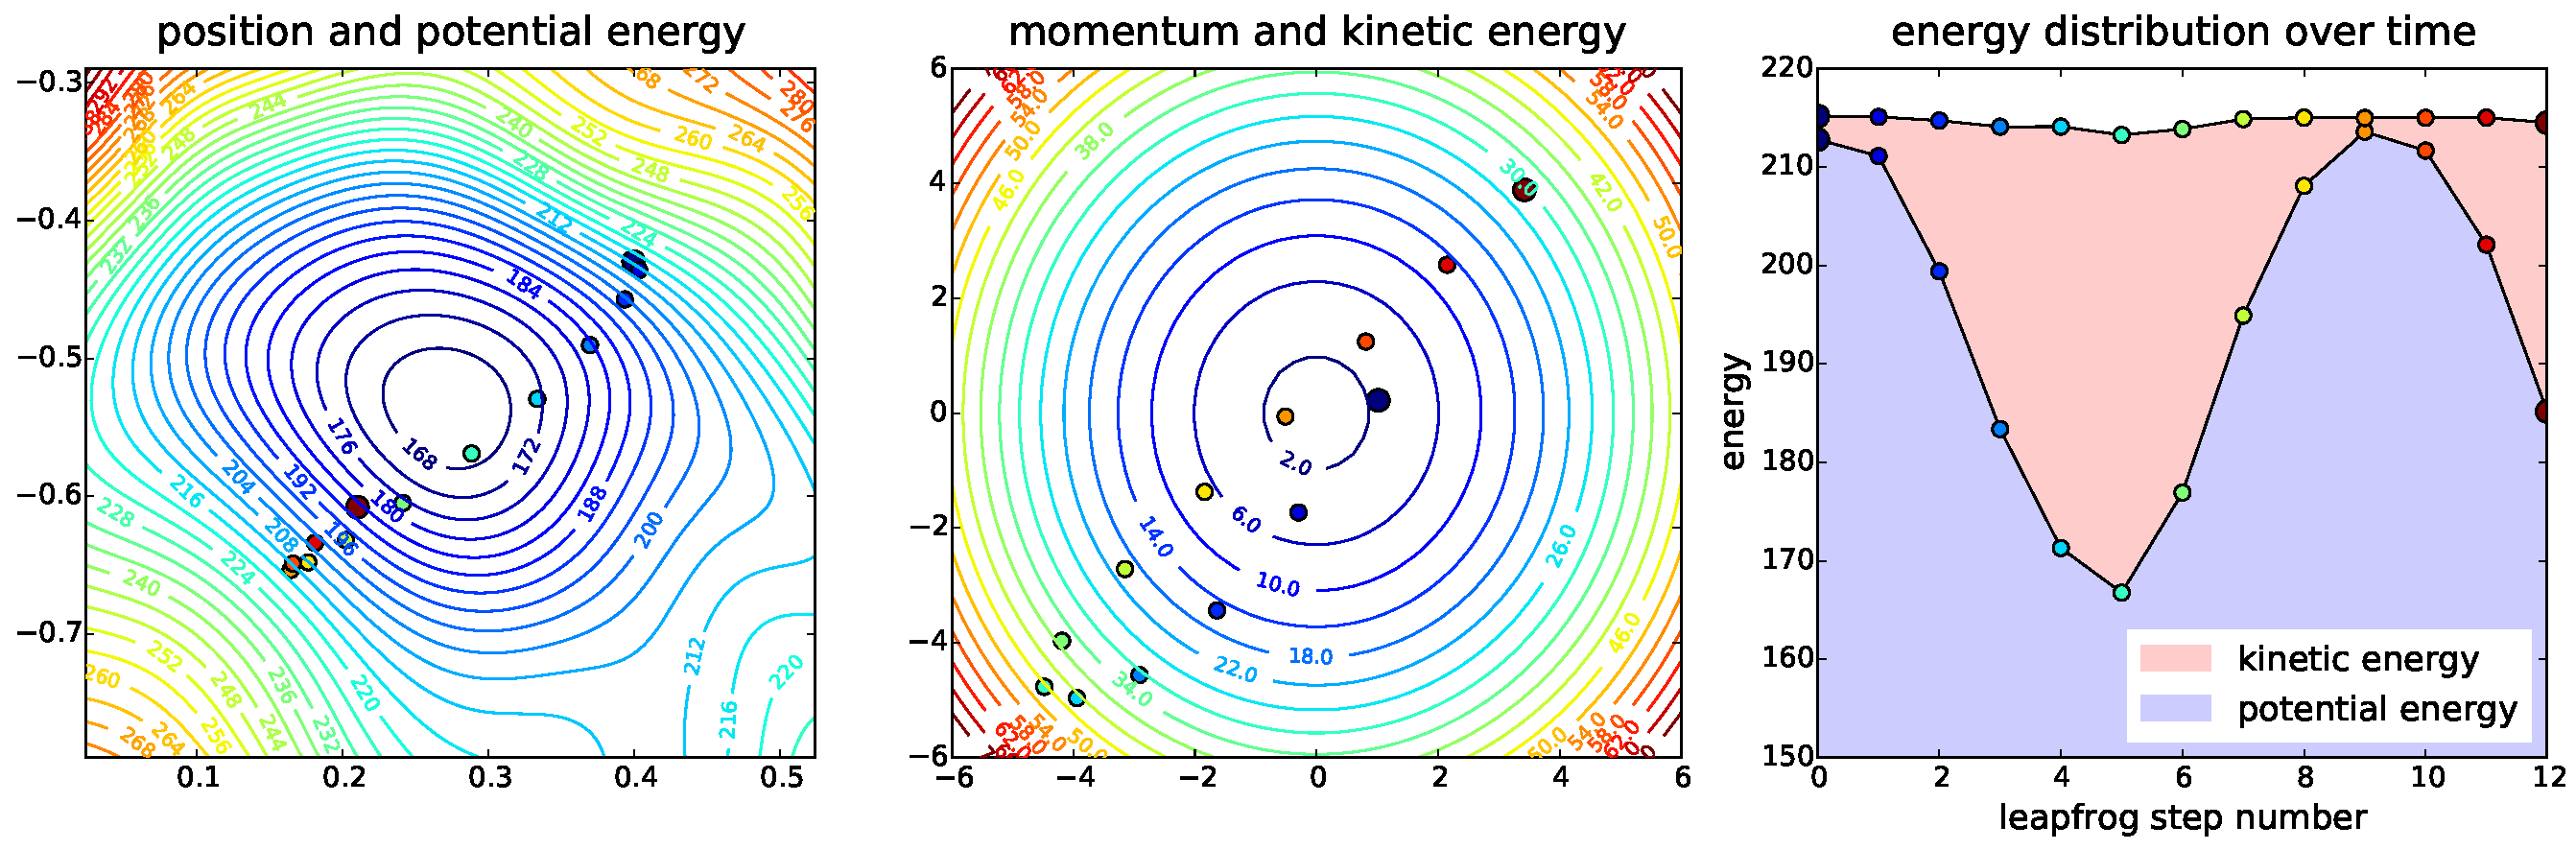
\includegraphics[width=2.05\columnwidth]{figures/hmc_motion_1hmc_12lf.pdf}
\caption{Dynamics of a particle under HD computed using the leapfrog method. Each computed point along the discretized trajectory is indicated by a separate color ranging from dark blue (starting point) to dark red (final point). The left plot shows the position of the particle with the prescribed potential energy represented by the contour plot. The centre plot depicts the momentum of the particle with the kinetic energy at each point indicated by the contours. In the plot on the right the energy distribution of the particle over time is given, with the potential energy in blue and the kinetic energy in red. Due to the discretization the total energy is not exactly conserved.}
\label{fig:HMC_MOTION_1hmc_12lf}
\end{figure*}

In such a physical system the kinetic energy is then given by $K(p) = p^T M^{-1} p /2$, where $M$ is called the mass matrix and in a physical context usually is $m I$, a scalar multiple of the identity. Here the scalar $m$ corresponds to the mass of the particle. With this kinetic energy we can retrieve Newton's equation of motion relating the acceleration $d^2q/dt^2$ to the force acting on a particle (given by $-\nabla U(q)$):
\begin{equation} \label{eq:NewtonsEquation}
\frac{d^2q}{dt^2} = M^{-1} \frac{dp}{dt} = - M^{-1} \frac{\partial H}{\partial q} = - M^{-1} \nabla U(q)
\end{equation}

The key advantage of HD over other formulations of classical dynamics is that analytic solutions to the above system have three crucial properties \parencite{Neal2011}:
\begin{itemize}
\item Reversibility: The mapping $T_s$ from the state $(q(t), p(t))$ at some time point $t$ to the state at $t+s$ ($s > 0$) is one-to-one and hence reversible. Thus by running time backwards, i.e.\ negating both time derivatives in Hamilton's equations, we can uniquely determine previous states.
\item Volume preservation: $T_s$ conserves volume in $(q, p)$-space, so applying it to some region of a certain volume results in a region of the same volume.
\item Conservation of the Hamiltonian: The Hamiltonian $H(q, p)$ is invariant with time, so $dH/dt = 0$.
\end{itemize}

All three of these properties would be useful in the application of the HMC algorithm, but due to the inevitable discretization of the differential equation not all of them can be preserved. The leapfrog method, which will be explained below, maintains reversibility and volume preservation and furthermore approximately conserves the Hamiltonian (see figure~\ref{fig:HMC_MOTION_1hmc_12lf}). This approximate conservation of the Hamiltonian makes it a so-called \textit{symplectic integrator}.

Given the step size $\epsilon$ the leapfrog method performs the following updates for $n \in \mathbb{N_0}$ starting from the initial state $(q^{(0)}, p^{(0)})$:
\begin{equation}
\begin{split}
p_i^{(n + 1/2)} &= p_i^{(n)} - \frac{\epsilon}{2} \frac{\partial U}{\partial q_i}(q^{(n)}) \\
q_i^{(n + 1)} &= q_i^{(n)} + \epsilon \frac{\partial K}{\partial p_i}(p^{(n + 1/2)}) \\
p_i^{(n + 1)} &= p_i^{(n + 1/2)} - \frac{\epsilon}{2} \frac{\partial U}{\partial q_i}(q^{(n + 1)})
\end{split}
\end{equation}
First a half-step for the momentum variables is computed, which is then used for a full position step. Finally, a second momentum half-step based on the updated position completes the leapfrog step. Since each of these updates is simply a shear transformation in $(q, p)$-space and therefore has a determinant of 1, a complete leapfrog step also has a determinant of 1 and is volume-conserving. If we perform multiple leapfrog steps, we can jump directly from $p_i^{(n + 1/2)}$ to $p_i^{(n + 3/2)}$ for greater efficiency.

With the usual choice for the kinetic energy $K(p) = p^T M^{-1} p /2$ and some manipulation of the above equations we can obtain an alternative formulation of the leapfrog method, which is more intuitive (but computationally more expensive):
\begin{equation}
\begin{split}
q^{(n + 1)} &= q^{(n)} + \epsilon M^{-1} p^{(n)}) + (\epsilon^2/2) M^{-1} F(q^{(n)}) \\
p^{(n + 1)} &= p^{(n)} + \epsilon (F(q^{(n)}) + F(q^{(n+1)}))/2,
\end{split}
\end{equation}
where $F(q) = - \nabla U(q)$ is the force acting on the particle at position $q$ due to the potential energy landscape. Since $M$ corresponds to the mass of the particle, $M^{-1} p$ gives its velocity and $M^{-1} F(q)$ its acceleration. From the first equation we see that the leapfrog method updates the position assuming motion under constant acceleration: $q(t) = q_0 + v_0 t + 1/2 a t^2$ with a initial position $q_0 = q^{(n)}$, initial velocity $v_0 = M^{-1} p^{(n)}$ and acceleration $a = M^{-1} F(q^{(n)})$. The second equation, which gives the momentum update, is simply a discretized version of the basic relationship $dp/dt = F$, i.e.\ force equals change of momentum, using the average of the forces at the start and the end point.

The local error of the leapfrog method, i.e.\ the error incurred in a single step, has order $\epsilon^3$; the global error, i.e.\ the error in the solution over a fixed time interval $L$, has order $\epsilon^2$. As a symplectic integrator the leapfrog method approximately conserves the Hamiltonian, so that the global error in the Hamiltonian, which is also order $\epsilon^2$, usually does not grow exponentially with the simulation length $L$ (with $\epsilon$ fixed) as it may for many other integration schemes \parencite{Neal2011}.

\subsection{The HMC algorithm}
\label{sec:HMCAlgorithmSection}
\subsubsection{Relating probability density to energy}
In order to apply HD within an MCMC method to sample from some target distribution, we need to derive appropriate energy functions. A key relationship in statistical mechanics is
\begin{equation}
P(s) = \frac{1}{Z} \exp \left(- \frac{E(s)}{T} \right),
\end{equation}
relating the probability density function $P(s)$ for observing a particle in state $s$ with the energy $E(s)$ of that state. Here, $T$ is the temperature of the system\footnote{$T$ is assumed here to be given in units such that the Boltzmann constant is 1.} and $Z$ is a normalization constant such that the total probability over all states equals 1. The distribution given by this probability density function is called the \textit{canonical distribution}.

By inverting this relationship we can derive the appropriate energy from any target distribution (w.l.o.g.\ setting $T=1$). The potential energy $U(q)$, whose canonical distribution has the target density $\tilde{P}(q)$, is thus given by $U(q) = -\log \left( \tilde{P}(q) \right) - \log Z$,
where we can drop the $\log Z$ term because energies only influence the particle motion through their derivatives. This also means that we do not need $\tilde{P}(q)$ to be normalized. A closer look at $U(q)$ reveals that it is the negative log-likelihood (NLL) of $\tilde{P}(q)$, which is frequently used as a minimization objective in machine learning. Therefore, this potential energy will promote motion towards low NLL points and thus the points proposed by motion simulation with this potential energy will tend to have a higher likelihood than those proposed by other methods.

For the simulation by HD the state of the system consists of the variable of interest $q$ plus an auxiliary momentum variable $p$ of the same size and so is given by the $2d$-dimensional $s = (q, p)$. With the potential energy $U(q)$ derived from the target distribution as described above, the Hamiltonian of this system is given by $H(q, p) = U(q) + K(p)$ for some kinetic energy $K(p)$ of our choice. Due to the additive nature of this Hamiltonian the joint canonical distribution of $(q, p)$ factorizes:
\begin{equation}
\begin{split}
p(q, p) &= \frac{1}{Z} \exp \left( -H(q, p) \right) \\
			&\propto \tilde{P}(q) \cdot \exp{(-K(p))}
\end{split}
\end{equation}

\subsubsection{Choice of kinetic energy}
In order to obtain a Markov chain, whose invariant distribution is the canonical distribution, some restrictions apply to the choice of kinetic energy \parencite{Betancourt2014}. In particular the corresponding canonical momentum distribution must have a mean of zero, since otherwise the resulting drift in the position variables makes convergence to the canonical distribution impossible. While it is possible to make the kinetic energy dependent on position in the Riemann Manifold Hamiltonian Monte Carlo method \parencite{Girolami2011}, this requires complicated modifications to the integrator and will not be considered here. \textcite{Betancourt2014} argue that there is little motivation to choose a kinetic energy other than the quadratic form from classical physics and in the following we will assume the usual choice for the kinetic energy
\begin{equation} \label{eq:KineticEnergy}
K(p) = p^T M^{-1} p/2
\end{equation}
for some positive definite mass matrix $M$. The corresponding canonical distribution (after normalization) $P_\textrm{kin}(p)$ is the multivariate Gaussian distribution with mean zero and covariance matrix $M$.

\subsubsection{The algorithm}
The HMC algorithm (see algorithm~\ref{alg:HMC}) produces the desired Markov chain \parencite{Neal2011}. There are two main steps in the algorithm: Firstly the simulation of HD using a reversible and volume-preserving integrator, e.g. the leapfrog method, and secondly a Metropolis-Hastings acceptance step to ensure the desired invariant distribution. Due to the momentum negation of the proposed state in the third step of the algorithm, the proposal distribution is symmetrical because of the reversibility of the integration method. As a result $\tilde{q}(\tilde{s}_t|s_{t-1}) = \tilde{q}(s_{t-1}|\tilde{s}_t)$ holds in the Metropolis-Hastings acceptance probability in equation~\eqref{eq:Metropolis-Hastings}, so the acceptance probability simplifies to
\begin{equation} \label{eq:AcceptanceProbability}
p_{\textrm{accept}}(s^*_{t-1}) = \min[1, \exp(-H(\tilde{s}_t) + H(s^*_{t-1}))].
\end{equation}

\begin{algorithm}
\caption{The HMC algorithm}\label{alg:HMC}
\begin{algorithmic}[1]
\Require Numeric integrator $HD(s)$ of Hamilton's equations simulating HD starting from state $s$ for a fixed length
\Require Current state $s_{t-1} = (q_{t-1}, p_{t-1})$
\State Sample new momentum $p^*_{t-1}$ from $P_\textrm{kin}$
\State Simulate HD starting from $s^*_{t-1} = (q_{t-1}, p^*_{t-1})$
\State Negate the momentum of the resulting state $s_\textrm{HD} = HD(s^*_{t-1})$ to obtain the proposed state $\tilde{s}_t = (q_\textrm{HD}, - p_\textrm{HD})$
\State Compute the acceptance probability $p_\textrm{accept}=p_\textrm{accept}(s^*_{t-1})$ as defined by equation~\eqref{eq:AcceptanceProbability}
\State Accept the move from $s^*_{t-1}$ to $\tilde{s}_t$ with probability $p_\textrm{accept}$
\State \textbf{Return} new state $s_t$
\end{algorithmic}
\end{algorithm}

It can be shown that this algorithm conserves the canonical distribution, which therefore also is the invariant distribution of the constructed Markov chain \parencite{Neal2011}. If the HD simulation was exact, then the Hamiltonian would be conserved, since negation of the momentum does not change the value of the Hamiltonian due to its symmetry. Therefore the acceptance probability would always be 1. However, numeric integrators cannot conserve the Hamiltonian exactly, necessitating the acceptance step. Still, for symplectic integrators, such as the leapfrog method, the numerical error usually remains bounded, allowing the rejection rate to be kept small even for long simulations.

\begin{figure*}[t]
\centering
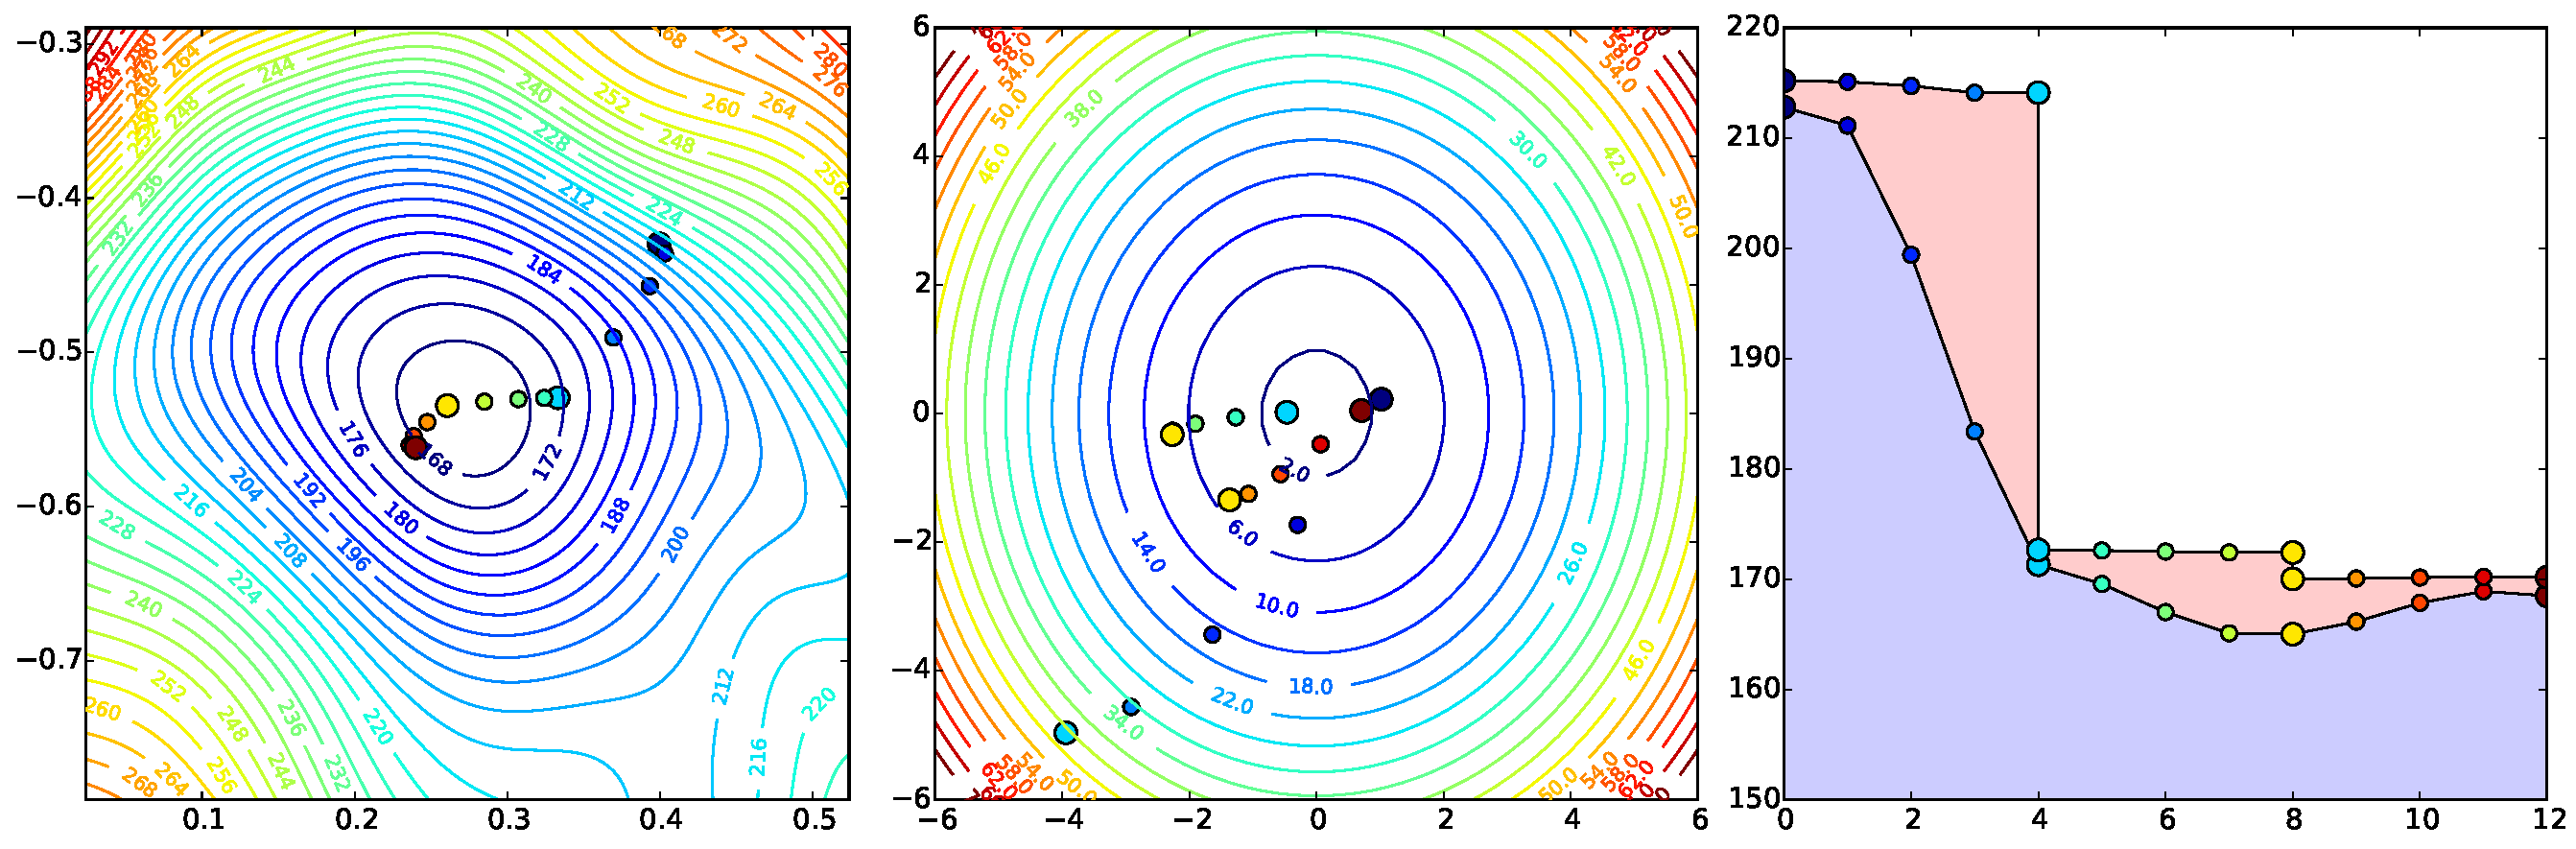
\includegraphics[width=2.05\columnwidth]{figures/hmc_motion_3hmc_04lf.pdf}
\caption{Evolution of a particle under the HMC algorithm with 3 HMC steps consisting of 4 leapfrog steps each. Each computed point along the trajectory is indicated by a separate color ranging from dark blue (starting point) to dark red (final point). Thicker dots highlight points, where momentum resampling was performed. The left plot shows the position of the particle with the prescribed potential energy represented by the contour plot. The centre plot depicts the momentum of the particle with the kinetic energy at each point indicated by the contours. Where the momentum was resampled, two identical dots are shown for the state before and after the resampling. In the plot on the right the energy distribution of the particle over time is given, with the potential energy in blue and the kinetic energy in red.}
\label{fig:HMC_MOTION_3hmc_04lf}
\end{figure*}

Due to the (approximate) conservation of the Hamiltonian during HD, the joint density $\exp \left( -H(q, p) \right)/Z$ of $(q,p)$ remains almost unchanged by steps 2 to 5 of the algorithm. Only the resampling of the momentum variable at the start of each HMC step allows large changes in the joint density. This can be seen in figure~\ref{fig:HMC_MOTION_3hmc_04lf}, where the evolution of a single particle is shown under the HMC algorithm. During the leapfrog steps the potential energy of the particle is partly converted to kinetic energy. With the newly drawn momentum the kinetic energy of the particle is smaller than before in this example leading to a decrease of its total energy. The sampled kinetic energy is given by $(1/2) p^T M^{-1} p$ (ignoring additive constants), which is $(1/2) \cdot \chi^2_d$-distributed for any $M$, if $p \sim P_\textrm{kin}(p)$. For the two-dimensional example in the figure this means that on average a particle gets a kinetic energy of 1 at the start of each HMC step, which could be converted into potential energy. Since the craters in the potential energy landscape are much deeper, particles are very unlikely to leave such a crater once they are caught inside.

Simulating an ensemble of particles illustrates how the convergence to the desired distribution happens in the HMC algorithm. In figure~\ref{fig:HMC_Effect_Illustration} particles were distributed according to some supposed distribution different from the desired distribution, which determines the energy landscape. After the first HMC step (bottom row of plots) the particles have mostly slid downhill, which can also be seen in the change in their potential energy (plots in the right column). Correspondingly, they have picked up kinetic energy, which will, however, be removed at the start of the next HMC step. In this way, the HMC steps initially reduce the amount of potential energy in the system corresponding to an increase of the likelihood of the particles w.r.t.\ the target distribution. By sampling a new momentum at the start of each HMC step, instead of for example setting it to 0 (in which case all the particles would gather at the low point of the potential energy), we ensure that the particles remain spread out and are eventually distributed according to the target distribution. 

\begin{figure*}[t]
\centering
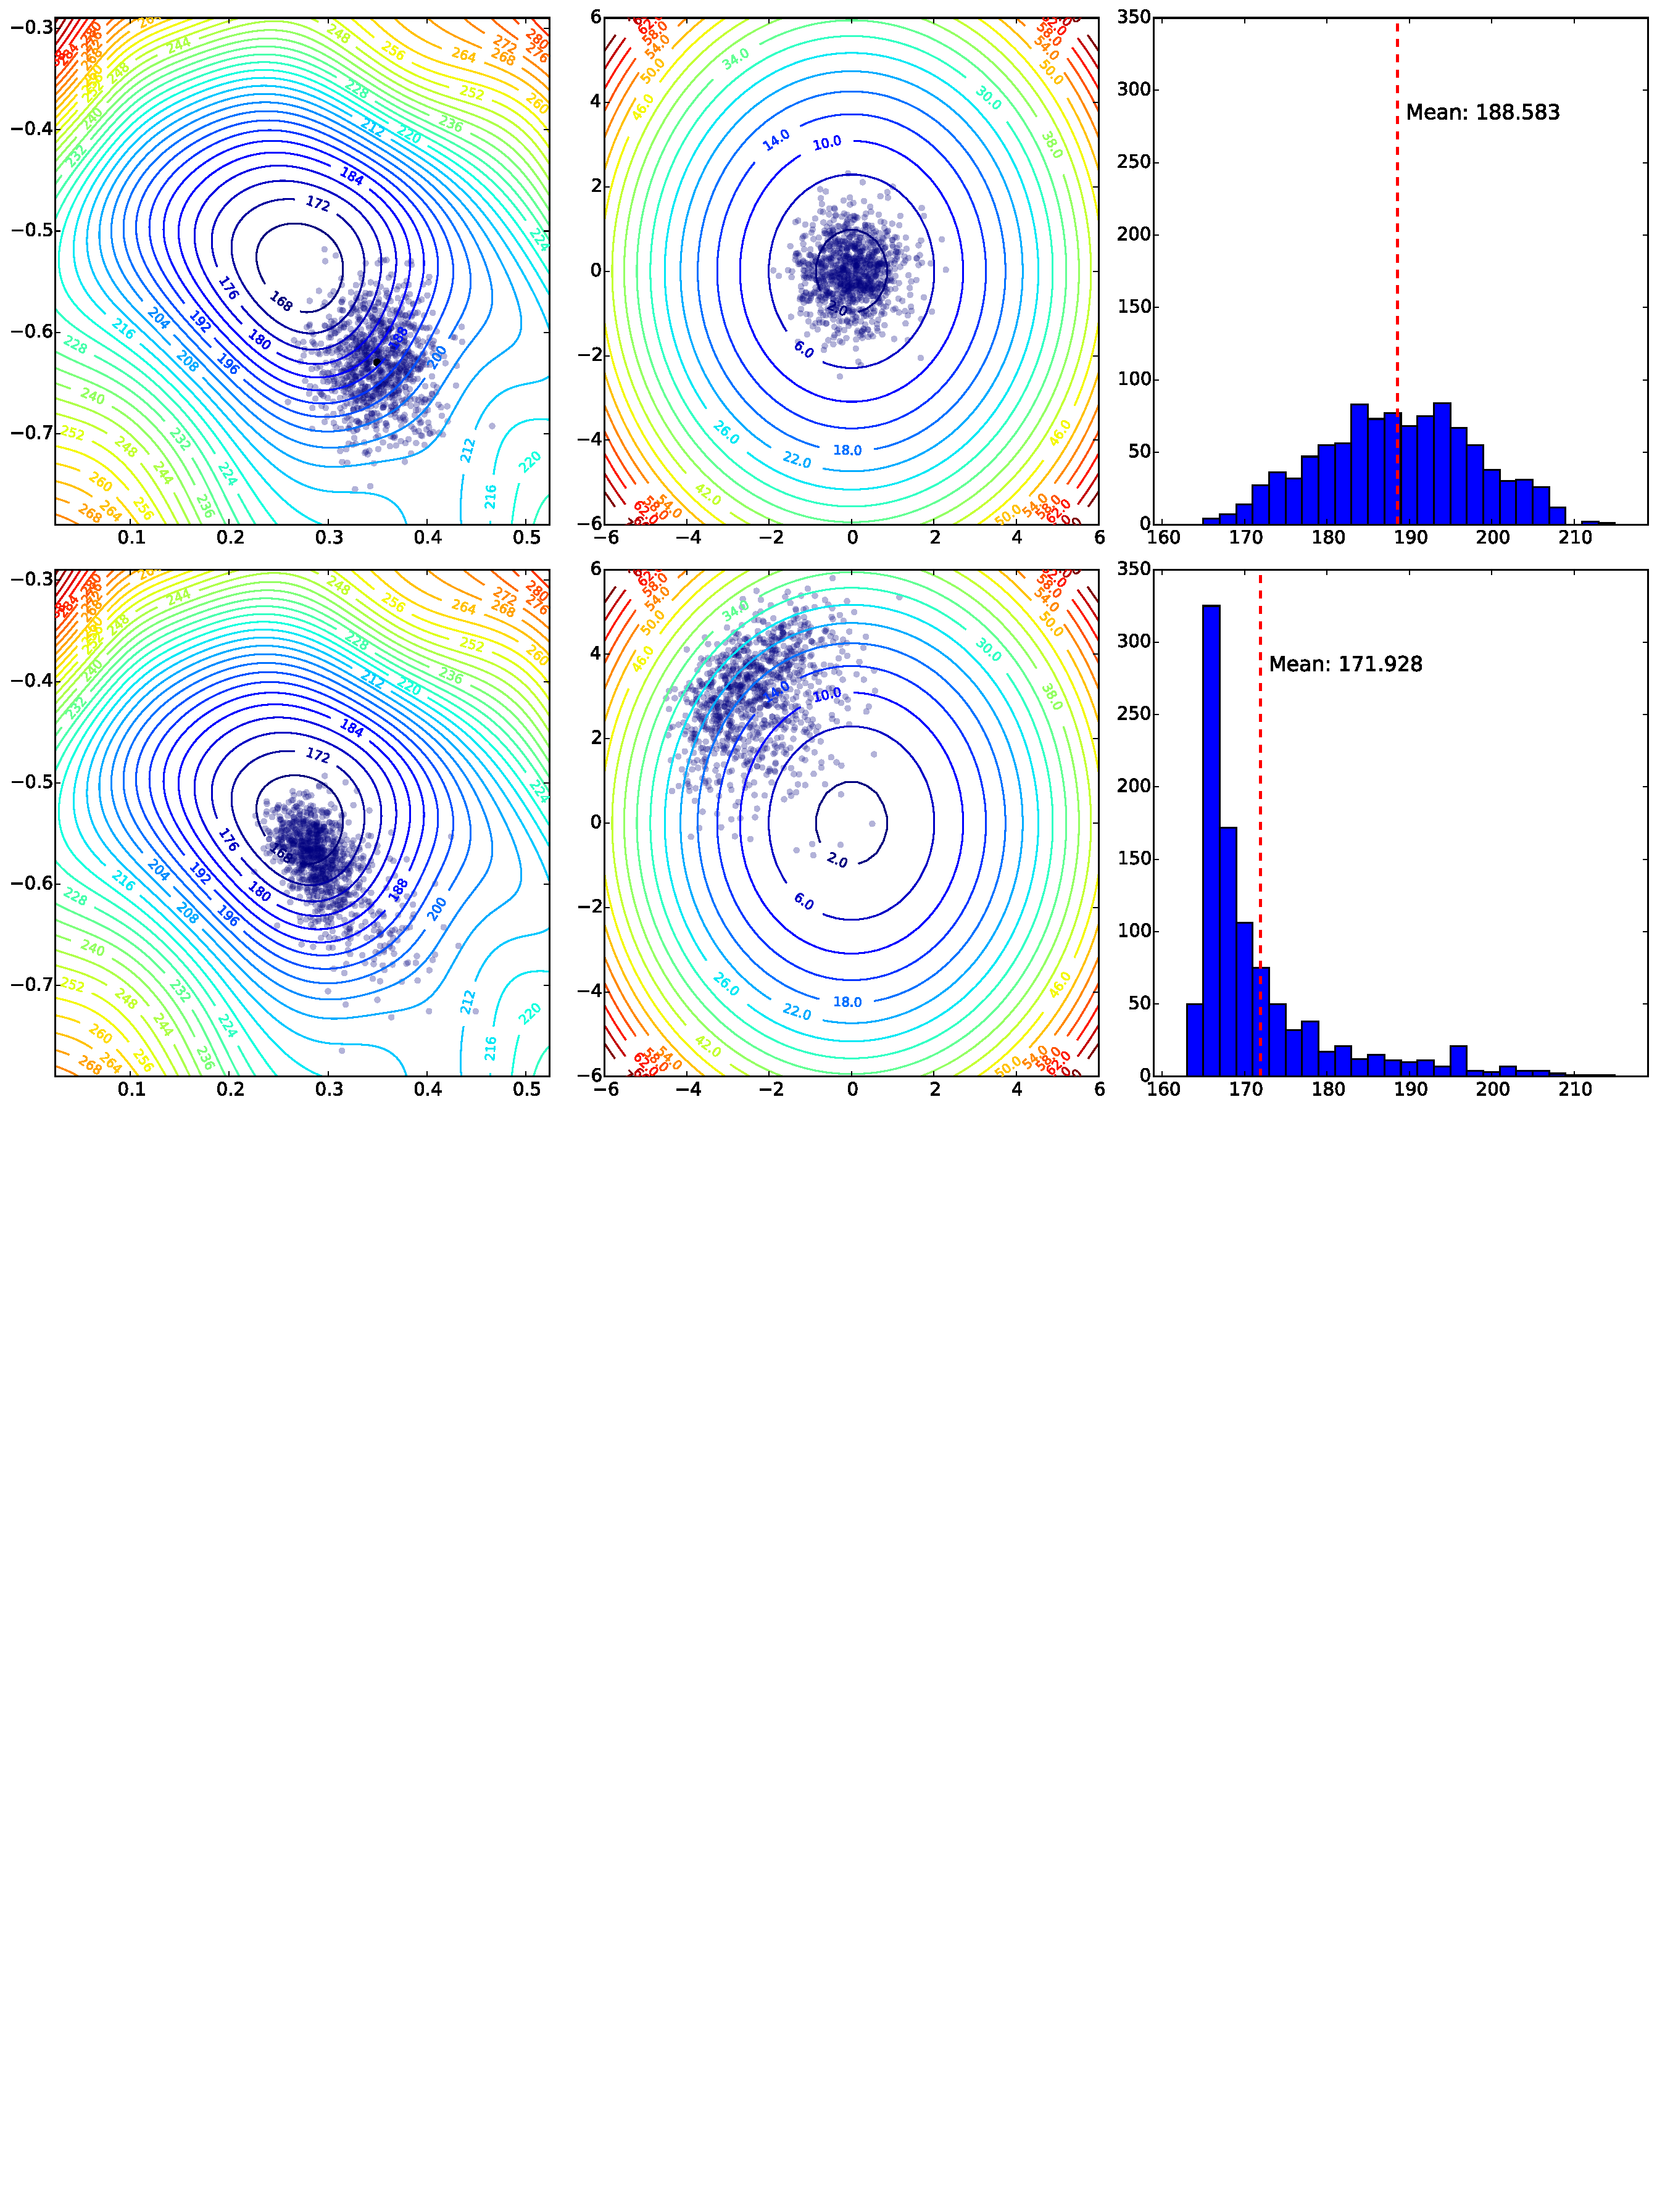
\includegraphics[width=2.05\columnwidth]{figures/hmcvi_distrib_example_top.pdf}
\caption{Evolution of an ensemble of 1000 particles under the HMC algorithm: The first row of plots shows the initial state of the system and the second row the state after an HMC step. The plots on the left give the positions of the particles with the prescribed potential energy represented by the contour plot. The centre plots depict the arrival momenta of the particles with the kinetic energy indicated by the contours. The right-hand plots show histograms of the potential energies of the particles.}
\label{fig:HMC_Effect_Illustration}
\end{figure*}

\subsection{Effect of the kinetic energy covariance matrix}
\label{sec:EffectOfKineticEnergyChoice}

For simplicity we restrict the kinetic energy (see eq.~\eqref{eq:KineticEnergy}) to be a positive-definite quadratic form, but not necessarily with a scalar multiple of the identity as mass matrix as the physical intuition of particle mass would suggest. A possible interpretation of such a "mass" matrix would be that the inertial mass of the particle, i.e.\ its resistance to change in velocity, is non-isotropic. In other words, the particle is more responsive to forces in some directions than in others. This somewhat non-physical freedom, however, has a very nice effect in the HMC algorithm: It allows an implicit rescaling of the $q$-space as explained below.

Such a rescaling can be very beneficial for the numerical solution, because the most restricted direction (with the most extreme changes in potential energy) limits the step length $\epsilon$ to be used in the discrete simulation. If a larger step length is used, the approximations of the energy surface used in the simulation are too coarse in the restricted direction and the discretization error becomes very large. As a result one may have to choose a very small step size, but this then limits the motion in the less restricted directions, where a larger step size would allow faster movement through the state space. Therefore, by rescaling the space we can achieve a more equal scaling in each direction, so that neither large errors nor slow exploration hamper the performance of the algorithm.

To see the connection between the mass matrix and the rescaling of $q$-space, assume the numerics of the dynamics w.r.t.\ the original variables $(q, p)$ were badly scaled when using the physically intuitive $K(p) = p^T p/2$ (taking $m=1$ for simplicity). Further suppose a transformation $q' = A^{-1} q$ with $p'=p$ and the same kinetic energy would yield a better scaling for some non-singular matrix $A$. Then the target distribution for $q'$ is given by $\tilde{P}'(q') = \tilde{P}(Aq')/|\det(A^{-1})|$ in terms of the original target distribution $\tilde{P}(q)$. Hence, the corresponding potential energy is $U'(q') = U(Aq')$, where we can drop the additive $\log(|\det(A^{-1})|)$ term. From Hamilton's equations (see equation~\eqref{eq:HamiltonsEquations}) for this system we get the following equations for the motion in terms of the original variables $(q, p)$:
\begin{equation}
\begin{split}
\frac{dq}{dt} &= A \frac{dq'}{dt} = Ap' = Ap \\
\frac{dp}{dt} &= \frac{dp'}{dt} = - \nabla U'(q') = - A^T \nabla U(q)
\end{split}
\end{equation}
The evolution of the position variable $q$ is thus given by (compare Newton's equation of motion~\eqref{eq:NewtonsEquation}):
\begin{equation} \label{eq:EvolutionQTransformed}
\frac{d^2q}{dt^2} = A \frac{dp}{dt} = - A A^T \nabla U(q)
\end{equation}

Now alternatively, let us consider the untransformed system, but with the kinetic energy $K''(p) = p^T A A^T p$. Then Hamilton's equation give us:
\begin{equation}
\begin{split}
\frac{dq}{dt} &= A A^T p \\
\frac{dp}{dt} &= - \nabla U(q),
\end{split}
\end{equation}
which results in the same evolution of the variable of interest $q$ as the direct transformation of $q$ above (compare equation~\eqref{eq:EvolutionQTransformed}). Regarding the evolution of $q$ these two approaches are thus identical (although the $p$ trajectories differ).

Introducing this transformation via the kinetic energy rather than transforming $q$ directly has the advantage, that we do not manipulate the variables of interest, which may be needed in their original form. Instead, we can achieve the same rescaling by modifying the auxiliary momentum variables, which do not have any external significance.

\subsection{Partial momentum update}
\label{sec:PartialMomentumUpdate}
If the number of leapfrog steps is small, subsequent points in the Markov chain generated by the HMC algorithm may be close to each other and highly correlated. This is especially obvious, if we imagine a flat plateau in the potential energy surface: Whatever momentum is sampled at the start of the HMC step, the simulated motion may frequently end at some other point still on the plateau, if the number of leapfrog steps is small. There the same may happen again, perhaps even bringing us back to the previous point, leading to an inefficient random-walk-like behaviour on this plateau.

To counter such a behaviour \textcite{Horowitz1991} proposed an extension to HMC, where the momentum is only partially updated. So instead of overwriting the momentum variable with a random sample from the canonical momentum distribution, the idea is to use a weighted sum of the current momentum and the newly drawn sample. By doing this the particle does not completely loose its current momentum after each HMC step, but continues in a similar direction as before. In the plateau example above, this means the particle is very unlikely to double back on its previous progress and will rather travel across the plateau in a directed fashion, avoiding the random-walk-like behaviour of the base HMC algorithm.

Some care must be taken in combining the current momentum $p_{t-1}$ with the new sample $p_\textrm{samp}$, because this momentum scrambling step must conserve the canonical distribution. This can be done by defining the updated momentum $p^*_{t-1}$ by
\begin{equation} \label{eq:partialMomentumUpdate}
p^*_{t-1} = \alpha \cdot p_{t-1} + \sqrt{1 - \alpha ^2} \cdot p_\textrm{sampled}
\end{equation}
for some $\alpha \in [-1, 1]$. In the converged chain both $p_{t-1}$ and $p_\textrm{sampled}$ are distributed according to the canonical distribution (Gaussian with mean zero and covariance matrix $M$), so $p^*_{t-1}$ will also be Gaussian and have mean zero. Since $p_{t-1}$ and $p_\textrm{sampled}$ are also independent of each other, the covariance is $\Cov(p^*_{t-1}) = \alpha^2 \cdot M + (1 - \alpha ^2) \cdot M = M$ as required.

\begin{algorithm}
\caption{The HMC algorithm with partial momentum updates}\label{alg:HMCWithPartial}
\begin{algorithmic}[1]
\Require Numeric integrator $HD(s)$ of Hamilton's equations simulating HD starting from state $s$ for a fixed length
\Require Current state $s_{t-1} = (q_{t-1}, p_{t-1})$
\State Sample new momentum $p_\textrm{samp}$ from $P_\textrm{kin}$
\State Update the momentum as in equation~\eqref{eq:partialMomentumUpdate} to obtain $p^*_{t-1}$
\State Simulate HD starting from $s^*_{t-1} = (q_{t-1}, p^*_{t-1})$
\State Negate the momentum of the resulting state $s_\textrm{HD} = HD(s^*_{t-1})$ to obtain the proposed state $\tilde{s}_t = (q_\textrm{HD}, - p_\textrm{HD})$
\State Compute the acceptance probability $p_\textrm{accept}=p_\textrm{accept}(s^*_{t-1})$ as defined by equation~\eqref{eq:AcceptanceProbability}
\State Accept the move from $s^*_{t-1}$ to $\tilde{s}_t$ with probability $p_\textrm{accept}$
\State Negate the momentum to obtain the new state $s_t$
\State \textbf{Return} new state $s_t$
\end{algorithmic}
\end{algorithm}

Algorithm~\ref{alg:HMCWithPartial} shows the steps in the improved version of the HMC algorithm for generating the next state of the Markov chain. Like the original HMC algorithm (algorithm~\ref{alg:HMC}), which can be recovered by setting $\alpha = 0$, this extension preserves the joint canonical distribution and thus yields a Markov chain with the required properties. Step 7, which is missing in the base version, is important for the case with partial momentum updates: If the proposed state was accepted, this step reverses the earlier momentum negation so that the particle keeps its direction. If the proposal was rejected, then it flips the momentum and the particle doubles back on itself. This can be clarified by combining steps 6 and 7:
\begin{equation} \label{eq:StateAfterAcceptReject}
s_t := \begin{cases} s_\textrm{HD} & \textrm{if accepted} \\ 
								(q_{t-1}, -p^*_{t-1}) & \textrm{if rejected}
					  \end{cases}
\end{equation}
For a better understanding, the order and used nomenclature of the states, which will be needed to derive the variational lower bound in section~\ref{sec:HMCVI}, are illustrated in figure~\ref{fig:HMC_schematic}.

\begin{figure}
\centering
\includegraphics{figures/hmc_illustration.tikz}
\caption{Flow chart illustrating the steps of the HMC algorithm with partial momentum updates.}
\label{fig:HMC_schematic}
\end{figure}

While the partial momentum update brings little benefit, if the number of leapfrog steps is large, it was reported to be beneficial for chains with shorter-than-optimal trajectories \parencite{Neal2011}. Because of computational limitations this will usually be the case in our application of HMC.